% Build from this directory with LuaLaTeX. See meta.md for the full command.
\documentclass{article}
\usepackage[paperwidth=841mm,paperheight=1189mm,margin=0mm]{geometry}
\usepackage[english]{babel}
\usepackage{fontspec,unicode-math}
\setmainfont{TeX Gyre Termes}
\setsansfont{IBM Plex Sans}
\newfontfamily\PosterSemi{IBMPlexSans-SemiBold.otf}
\setmathfont{TeX Gyre Termes Math}
\usepackage{graphicx,booktabs,tabularx,array,ragged2e}
\usepackage{tikz,pgfplots}
\usetikzlibrary{arrows.meta,calc,positioning}
\pgfplotsset{compat=1.18}
\definecolor{navy}{HTML}{1F3050}
\definecolor{teal}{HTML}{187E8A}
\definecolor{burgundy}{HTML}{600030}
\definecolor{pale}{HTML}{F3F4F7}
\usepackage[unicode,colorlinks=true,urlcolor=navy]{hyperref}
\hypersetup{
  pdftitle={Can ten qubits finish your sentence?},
  pdfauthor={Ethan Bandasack, Malo Leroy, Thierry Zhang},
  pdfsubject={Quantum semantics and language prediction under classical controls},
  pdfkeywords={quantum semantics, Hamiltonian, language model, classical controls, poster}
}
\pagestyle{empty}
\setlength{\parindent}{0pt}
\setlength{\parskip}{0pt}
\hyphenpenalty=10000
\exhyphenpenalty=10000
\newcommand{\bodyfont}{\rmfamily\fontsize{28}{35}\selectfont}
\newcommand{\smallfont}{\rmfamily\fontsize{24}{30}\selectfont}
\newcommand{\chartfont}{\sffamily\fontsize{24}{29}\selectfont}
\newcommand{\headingfont}{\sffamily\bfseries\fontsize{36}{43}\selectfont}
\newcommand{\putblock}[4]{%
  \node[anchor=north west,inner sep=0pt,outer sep=0pt,text width=#3mm,align=left]
    at ([xshift=#1mm,yshift=-#2mm]current page.north west) {\RaggedRight#4};}
\newcommand{\sectiontitle}[4]{%
  \putblock{#1}{#2}{#3}{{\headingfont\color{navy}#4}}}
\newcommand{\ruleat}[3]{%
  \draw[navy!22,line width=1.5pt]
    ([xshift=#1mm,yshift=-#2mm]current page.north west) -- ++(#3mm,0);}
\pgfplotsset{poster/.style={
  axis lines=left,axis line style={navy,line width=2.2pt},
  tick style={navy,line width=2pt},tick label style={font=\chartfont},
  label style={font=\chartfont},grid style={navy!12,line width=1pt},
  major tick length=3mm,minor tick num=0,clip=false,
  every axis plot/.append style={line width=3pt},scaled ticks=false}}
\begin{document}
\null
\begin{tikzpicture}[remember picture,overlay]
	% Unmodified supplied logos, on a white strip at the top.
	\putblock{30}{35}{108}{
\includegraphics[width=108mm]{Mail attachments/logoCS-UPSaclay.png}}
	\putblock{183}{28}{105}{
\includegraphics[width=105mm]{logos/L2S_logo.png}}
	\putblock{343}{5}{145}{
\includegraphics[width=145mm]{Mail attachments/LogoEUGLOH_lettering_transparent.png}}
	\putblock{554}{24}{257}{
\includegraphics[width=257mm]{Mail attachments/EN Co-Funded by the EU_POS.png}}
	\fill[navy] ([yshift=-87mm]current page.north west)
	rectangle ([yshift=-231mm]current page.north east);
	\fill[teal] ([yshift=-231mm]current page.north west)
	rectangle ([yshift=-234mm]current page.north east);
	\putblock{30}{102}{781}{{\sffamily\bfseries\fontsize{96}{108}\selectfont\color{white}
				Can ten qubits finish your sentence?}}
	\putblock{30}{151}{781}{{\PosterSemi\fontsize{56}{66}\selectfont\color{white}
				Quantum language models under classical controls}}
	\putblock{30}{188}{781}{{\sffamily\fontsize{32}{39}\selectfont\color{white}
				Ethan Bandasack\qquad Malo Leroy\qquad Thierry Zhang}}
	\putblock{30}{208}{781}{{\sffamily\fontsize{26}{32}\selectfont\color{white}
				CentraleSupélec, Université Paris-Saclay, L2S, Gif-sur-Yvette, France\quad
				Supervisor: Zeno Toffano}}
	\sectiontitle{30}{253}{235}{1\quad Meaning as operators}
	\putblock{30}{278}{235}{{\bodyfont
				Quantum semantics encodes meaning relations as Pauli operators [1,2].}}
	\putblock{33}{336}{229}{% Editable semiotic square, adapted from the report. Example category: temperature.
\begin{tikzpicture}[x=1mm,y=1mm,>=Latex,
		term/.style={anchor=center,font=\bodyfont,align=center,inner sep=1mm,text=navy},
		rel/.style={anchor=center,font=\chartfont,fill=white,inner sep=1mm,text=teal},
		edge/.style={teal,line width=2.8pt}]
	\path[use as bounding box] (-8,-14) rectangle (221,78);
	\node[term] (a) at (30,63) {hot};
	\node[term] (b) at (183,63) {cold};
	\node[term] (nb) at (30,0) {not cold};
	\node[term] (na) at (183,0) {not hot};
	\draw[edge,<->] (a) -- node[rel,above=2mm] {opposition $\sigma_z$} (b);
	\draw[edge,->] (a) -- node[rel,rotate=90,above=2mm] {inclusion $\sigma_y$} (nb);
	\draw[edge,->] (b) -- (na);
	\draw[edge,<->] (a) -- (na);
	\draw[edge,<->] (b) -- (nb);
	\node[rel] at (106.5,31.5) {negation $\sigma_x$};
	\draw[navy!40,line width=2pt,dashed,<->] (nb) -- (na);
\end{tikzpicture}
}
	\putblock{30}{434}{235}{{\smallfont
				The semiotic square motivates our work.
				Prediction tests trainability, not semantic relations.}}
	\sectiontitle{291}{253}{520}{2\quad Purpose and methods}
	\putblock{291}{278}{520}{{\bodyfont
				Does quantum evolution improve token prediction under classical controls
				with equal inputs, targets and update budgets?}}
	\putblock{291}{315}{520}{{\chartfont
\renewcommand{\arraystretch}{1.15}
\begin{tabularx}{\dimexpr\linewidth-2mm\relax}{@{}p{142mm}p{154mm}X@{}}
	\toprule
	\textbf{Model family}      & \textbf{Readout}    & \textbf{Control}          \\
	\midrule
	QCSE, 10 / 14 qubits [3]   & Thresholded bits    & Constant prior            \\
	Hybrid, 8 qubits           & Classical word head & Identity circuit, MLP [4] \\
	Hamiltonian, 8 / 10 qubits & Born probabilities  & Dephased state, MLP       \\
	\bottomrule
\end{tabularx}\par}
\vspace{5mm}
{\smallfont\textbf{Final model:} 9 token qubits + 1 auxiliary, 3 Hamiltonian stages.\par}
\vspace{4mm}
\begin{tikzpicture}[x=1mm,y=1mm,>=Latex,
		stage/.style={anchor=center,font=\chartfont,align=center,inner sep=3mm,minimum height=19mm},
		link/.style={->,navy,line width=2.8pt}]
	\node[stage,anchor=west] (c) at (0,0) {Context\\128 tokens};
	\node[stage] (p) at (171,0) {Last-token prior\\$\lvert\psi_0(C)\rangle$};
	\node[stage,draw=teal,line width=2.5pt,text=teal] (u) at (322,0)
	{Learned evolution\\$U_\theta(C)$};
	\node[stage,anchor=east] (b) at (520,0) {Born readout\\$p_\theta(y\mid C)$};
	\draw[link] (c) -- (p); \draw[link] (p) -- (u); \draw[link] (u) -- (b);
	\draw[link,dashed] (c.south) -- ++(0,-11) -| (u.south);
	\node[anchor=center,font=\chartfont,text=navy,fill=white,inner sep=1mm]
	at (177,-20) {Classical context pooling};
\end{tikzpicture}
}
	\putblock{291}{446}{520}{{\smallfont
				Noiseless simulation. Training-only vocabulary/statistics. Grouped splits.
				Hamiltonian checkpoints: minimum validation NLL. Hybrid: last epoch. Capacities/schedules differ.\\
				MLP: multilayer perceptron. NLL: negative log-likelihood (lower is better).}}
	% Results occupy the largest continuous region of the poster.
	\fill[pale] ([xshift=18mm,yshift=-489mm]current page.north west)
	rectangle ([xshift=-18mm,yshift=-990mm]current page.north east);
	\sectiontitle{30}{502}{781}{3\quad Results: classical controls lead the main comparisons}
	\putblock{30}{533}{370}{{\headingfont\fontsize{34}{41}\selectfont\color{navy}
				A\quad A constant guess beats\\QCSE's published metric}}
	\putblock{441}{533}{370}{{\headingfont\fontsize{34}{41}\selectfont\color{navy}
				B\quad Removing the circuit\\changes little}}
	\putblock{30}{579}{370}{% Values: report Appendix, QCSE miniature audit. Each bar names its model.
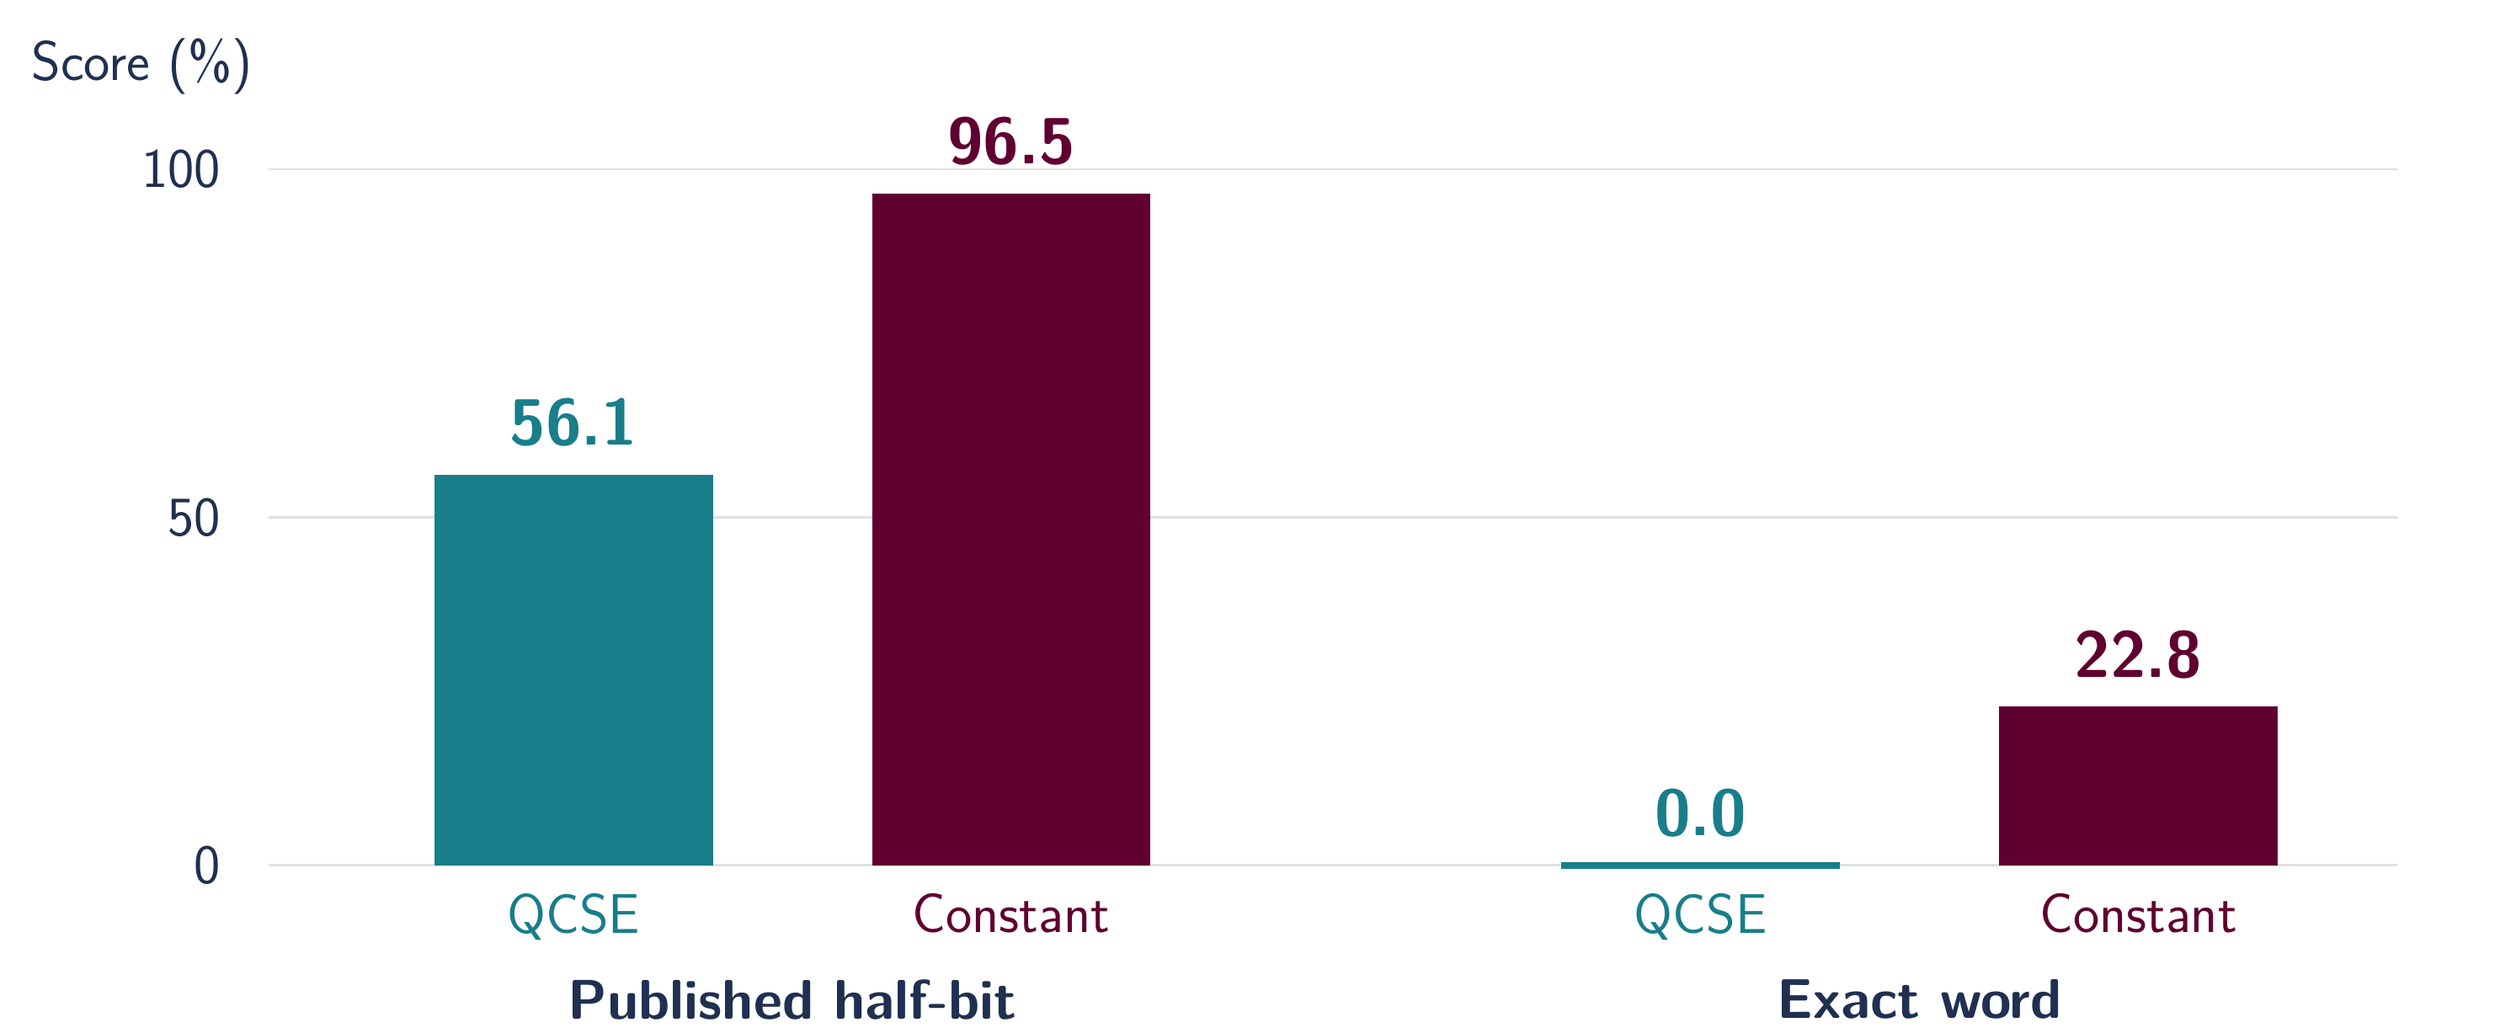
\begin{tikzpicture}[x=1mm,y=1mm]
	\path[use as bounding box] (0,-21) rectangle (370,127);
	\foreach \v in {0,50,100}{
			\draw[navy!15,line width=1pt] (37,{1.05*\v}) -- (358,{1.05*\v});
			\node[anchor=east,font=\chartfont,text=navy] at (31,{1.05*\v}) {\v};}
	\node[anchor=south west,font=\chartfont,text=navy] at (0,115) {Score (\%)};
	\fill[teal] (62,0) rectangle (104,58.905);
	\fill[burgundy] (128,0) rectangle (170,101.325);
	\draw[teal,line width=3pt] (232,0) -- (274,0);
	\fill[burgundy] (298,0) rectangle (340,23.94);
	\foreach \xx/\yy/\val/\col in {83/58.905/56.1/teal,149/101.325/96.5/burgundy,253/0/0.0/teal,319/23.94/22.8/burgundy}{
			\node[anchor=south,font=\sffamily\bfseries\fontsize{28}{32}\selectfont,text=\col]
			at (\xx,{\yy+3}) {\val};}
	\foreach \xx/\lab/\col in {83/QCSE/teal,149/Constant/burgundy,253/QCSE/teal,319/Constant/burgundy}{
			\node[anchor=north,font=\chartfont,text=\col] at (\xx,-3) {\lab};}
	\node[anchor=north,font=\chartfont\bfseries,text=navy] at (116,-16) {Published half-bit};
	\node[anchor=north,font=\chartfont\bfseries,text=navy] at (286,-16) {Exact word};
\end{tikzpicture}
}
	\putblock{441}{579}{370}{% Final benchmark: circuit is CRZ for left-only, ZZ for both sides.
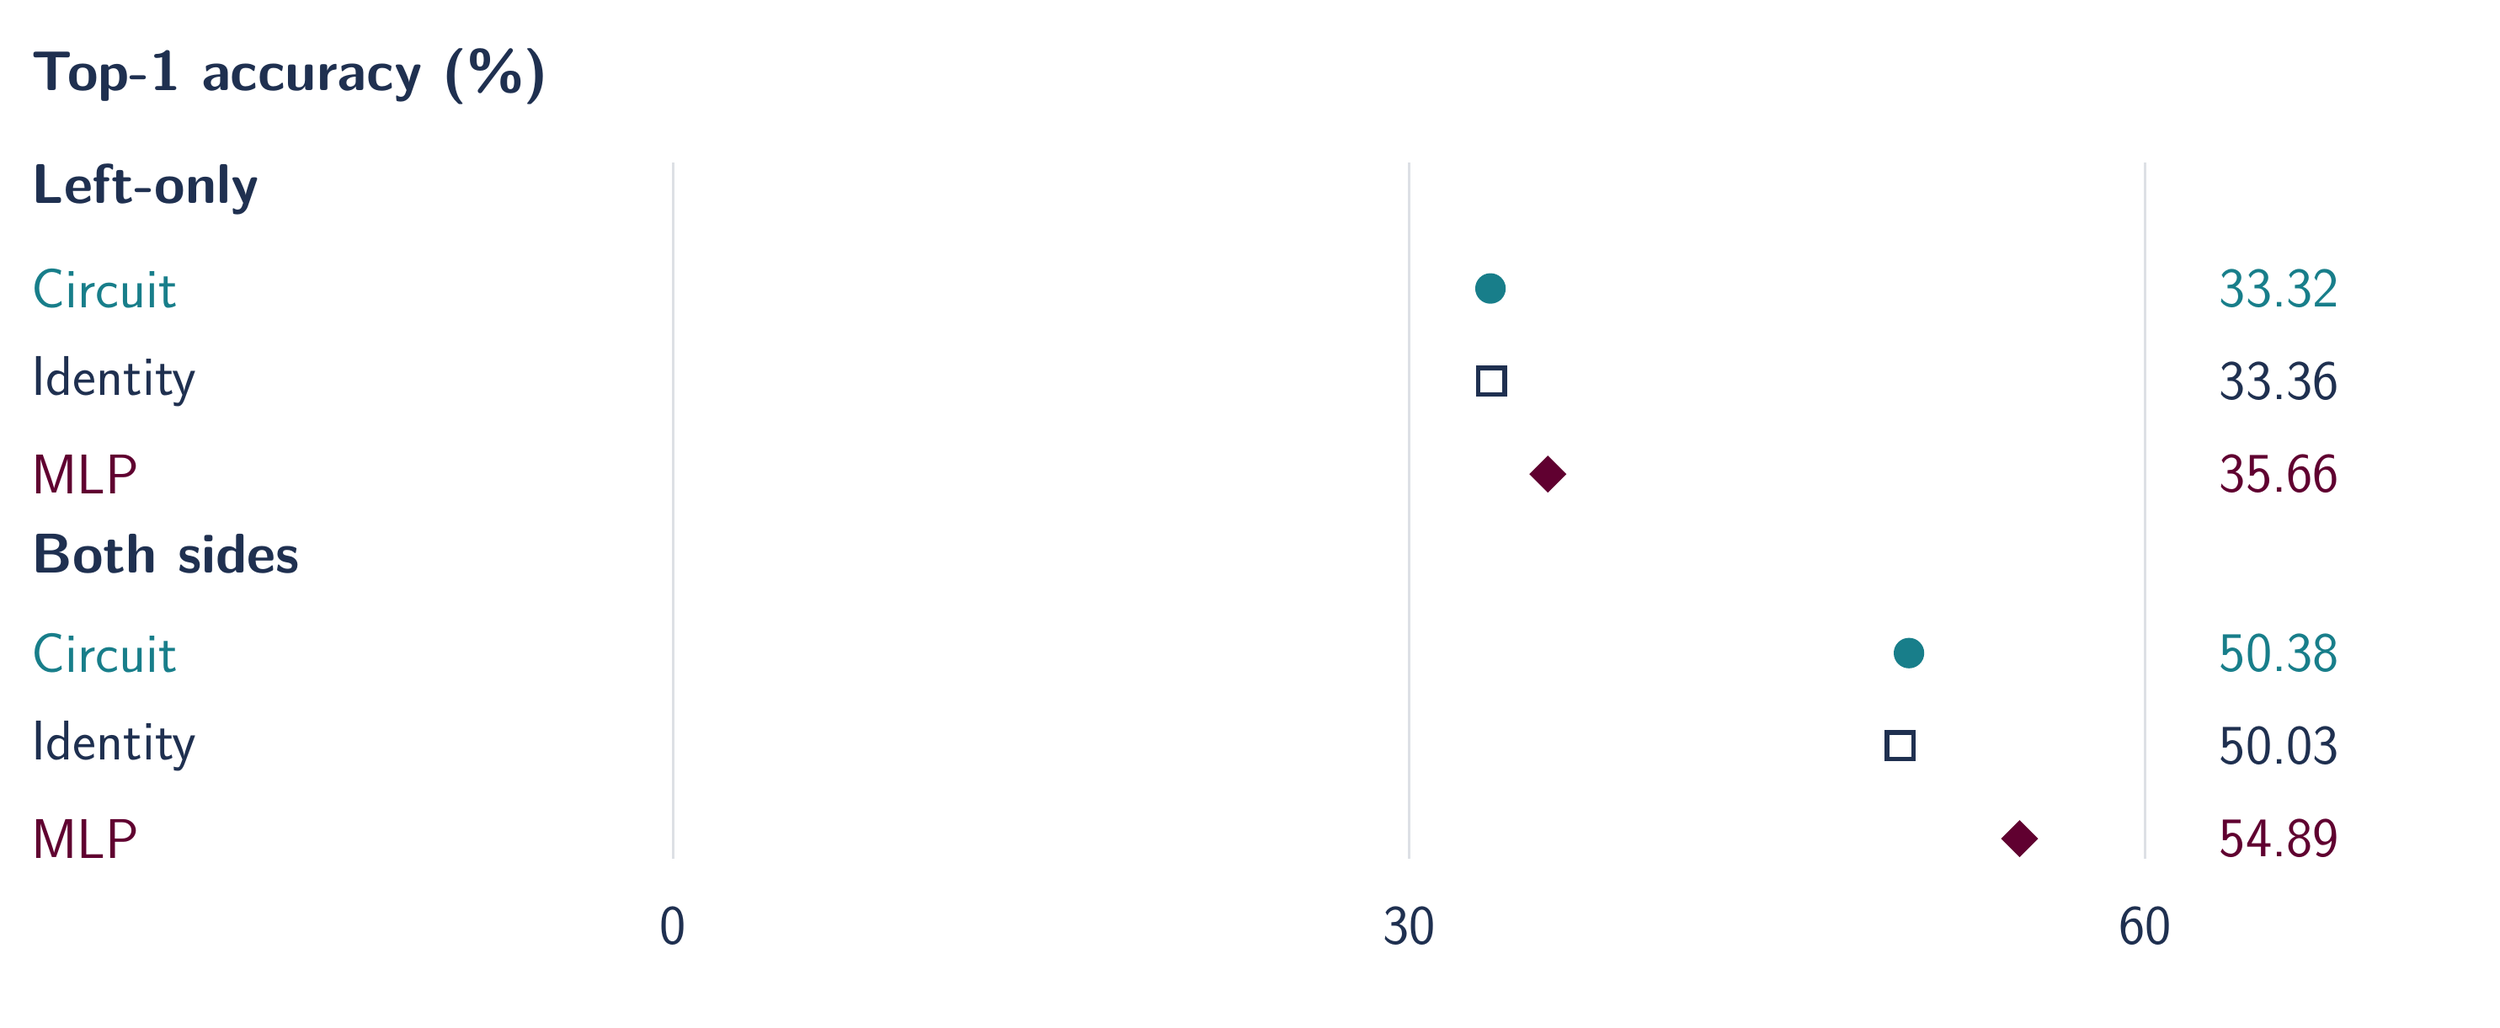
\begin{tikzpicture}[x=1mm,y=1mm]
	\path[use as bounding box] (0,-21) rectangle (370,127);
	\node[anchor=west,font=\chartfont\bfseries,text=navy] at (0,119) {Top-1 accuracy (\%)};
	\foreach \v in {0,30,60}{
			\draw[navy!15,line width=1pt] ({98+3.7*\v},1) -- ({98+3.7*\v},106);
			\node[anchor=north,font=\chartfont,text=navy] at ({98+3.7*\v},-5) {\v};}
	\node[anchor=west,font=\chartfont\bfseries,text=navy] at (0,102) {Left-only};
	\node[anchor=west,font=\chartfont\bfseries,text=navy] at (0,47) {Both sides};
	\foreach \yy/\val/\lab in {87/33.32/Circuit,32/50.38/Circuit}{
			\node[anchor=west,font=\chartfont,text=teal] at (0,\yy) {\lab};
			\fill[teal] ({98+3.7*\val},\yy) circle[radius=2.3mm];
			\node[anchor=west,font=\chartfont,text=teal] at (330,\yy) {\val};}
	\foreach \yy/\val in {73/33.36,18/50.03}{
			\node[anchor=west,font=\chartfont,text=navy] at (0,\yy) {Identity};
			\draw[navy,line width=2pt,fill=white] ({98+3.7*\val-2},\yy-2) rectangle ++(4,4);
			\node[anchor=west,font=\chartfont,text=navy] at (330,\yy) {\val};}
	\foreach \yy/\val in {59/35.66,4/54.89}{
			\node[anchor=west,font=\chartfont,text=burgundy] at (0,\yy) {MLP};
			\fill[burgundy] ({98+3.7*\val},\yy+2.8) -- ++(2.8,-2.8) -- ++(-2.8,-2.8) -- ++(-2.8,2.8) -- cycle;
			\node[anchor=west,font=\chartfont,text=burgundy] at (330,\yy) {\val};}
\end{tikzpicture}
}
	\putblock{30}{734}{370}{{\smallfont
				Half-bit accepts 5/10 matching bits. Audit: 57 test targets.}}
	\putblock{441}{734}{370}{{\smallfont
				Identity keeps the classical head. Context: 4 left words or 2 on each side.
				2 seeds, 252,120 validation targets (CRZ / $ZZ$, respectively).}}
	\ruleat{30}{780}{781}
	\putblock{30}{795}{781}{{\headingfont\fontsize{34}{41}\selectfont\color{navy}
				C\quad The Hamiltonian learns, but the MLP leads}}
	\putblock{30}{830}{512}{% Selected design milestones, not epochs. Full-precision data: source-data.csv.
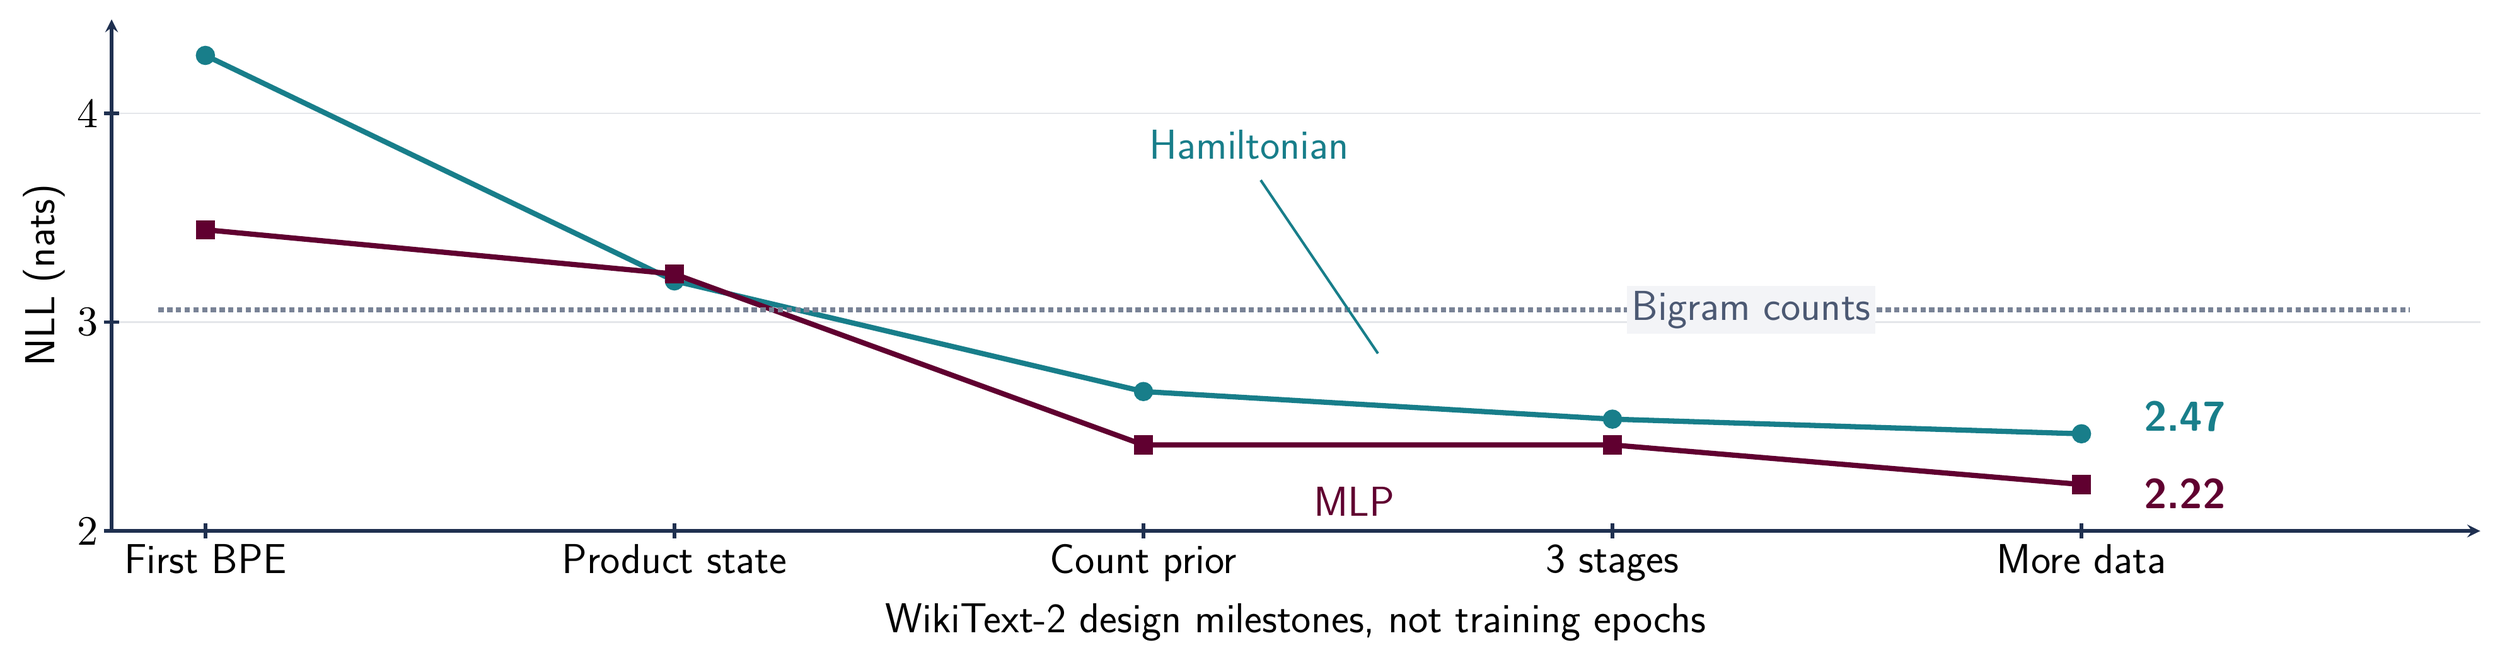
\begin{tikzpicture}
	\begin{axis}[poster,
			width=493mm,height=119mm,scale only axis=false,
			xmin=0.8,xmax=5.85,ymin=2.0,ymax=4.45,
			ytick={2,3,4},xtick={1,2,3,4,5},
			xticklabels={First BPE,Product state,Count prior,3 stages,More data},
			xticklabel style={font=\chartfont,align=center},
			ylabel={NLL (nats)},ymajorgrids=true,xmajorgrids=false,
			xlabel={WikiText-2 design milestones, not training epochs},
			xlabel style={font=\chartfont,yshift=-2mm}]
		\addplot[teal,mark=*,mark size=4pt] coordinates {
				(1,4.2773) (2,3.1975) (3,2.66776) (4,2.53554) (5,2.46546)};
		\addplot[burgundy,mark=square*,mark size=4pt] coordinates {
				(1,3.4424) (2,3.2306) (3,2.41207) (4,2.41207) (5,2.22277)};
		\addplot[navy!60,densely dashed,domain=0.9:5.7,samples=2] {3.0593};
		\node[font=\chartfont,text=teal,anchor=west] at (axis cs:3.0,3.85) {Hamiltonian};
		\draw[teal,line width=1.5pt] (axis cs:3.25,3.68) -- (axis cs:3.5,2.85);
		\node[font=\chartfont,text=navy!80,anchor=west,fill=pale,inner sep=1mm]
		at (axis cs:4.03,3.0593) {Bigram counts};
		\node[font=\chartfont,text=burgundy,anchor=west] at (axis cs:3.35,2.14) {MLP};
		\node[font=\chartfont\bfseries,text=teal,anchor=west] at (axis cs:5.12,2.55) {2.47};
		\node[font=\chartfont\bfseries,text=burgundy,anchor=west] at (axis cs:5.12,2.18) {2.22};
	\end{axis}
\end{tikzpicture}
}
	\putblock{573}{836}{224}{{\sffamily\bfseries\fontsize{57}{64}\selectfont\color{burgundy}
				0.24 nats}}
	\putblock{573}{862}{224}{{\bodyfont
				lower MLP validation NLL.\\
				Final comparison: 3 seeds, 4,096 targets.}}
	\putblock{573}{912}{224}{{\smallfont
				\textbf{Born-sampled continuation}\\
				Prompt: \textquotedblleft The history of \textquotedblright\\
				\textquotedblleft its first game ream , butvarBan7\textquotedblright\\[3mm]
				Generation remains incoherent.}}
	\putblock{50}{974}{490}{{\smallfont
				512 subword tokens. Vertical pairs share data and exposure.
				Last 3 points: 3-seed means.}}
	\sectiontitle{30}{1008}{235}{4\quad Interpretation}
	\putblock{30}{1032}{235}{{\smallfont
				Coherent vs separately trained dephased input:
				6.76\% vs 5.71\% one-draw success (word-level test).
				Entanglement benefit unproven.}}
	\putblock{291}{1008}{520}{{\headingfont\color{navy}5\quad Conclusions}}
	\putblock{291}{1032}{520}{{\sffamily\bfseries\fontsize{36}{44}\selectfont\color{navy}
				No quantum advantage emerged in these experiments.\\
				Check the metric and the classical control.}}
	\putblock{291}{1072}{520}{{\smallfont
				Limits: simulation, few seeds, reused WikiText validation, test unscored.
				Next: test semantic relations.}}
	\ruleat{30}{1113}{781}
	\putblock{30}{1122}{495}{{\rmfamily\fontsize{20}{25}\selectfont
				\textbf{References}\quad
				[1] Galofaro et al. (2018). A quantum-based semiotic model for textual semantics.
				\emph{Kybernetes} 47, 307--320.\newline
				{}[2] Dubois \& Toffano (2026). On Quantum Relations. \emph{Entropy} 28, 522.\newline
				{}[3] Varmantchaonala et al. (2026). QCSE. arXiv:2509.05729v2.\newline
				{}[4] Bengio et al. (2003). A Neural Probabilistic Language Model. \emph{JMLR} 3, 1137--1155.}}
	\putblock{558}{1122}{253}{{\rmfamily\fontsize{20}{25}\selectfont
				\textbf{AI \& One Health Co-creation workshop}\\
				20 November 2026\quad Group 21\\
				\textbf{Declarations of interest: None.}\\
				LLM assistance: literature, code, drafting.\\
				Numerical results verified.}}
\end{tikzpicture}
\end{document}
